\documentclass[conference]{IEEEtran}
\usepackage{fontspec}
\setmainfont{Times New Roman}
\setsansfont{Arial}
\setmonofont{Menlo}
\usepackage{amsmath}
\usepackage{graphicx}
\usepackage{booktabs}
\usepackage{url}

\title{A Qualitative Study of Block-Based Work Stealing on Apple Silicon}

\author{\IEEEauthorblockN{Muhammad Umar Aibak}
\IEEEauthorblockA{School of Software Technology, Dalian University of Technology\\
\texttt{uaibak008@mail.dlut.edu.cn}}}

\begin{document}
\maketitle

\begin{abstract}
Work stealing lets an idle worker take tasks from a busier worker, but the coordination can slow the worker that owns the queue. Block-based Work Stealing (BWoS) reduces this cost by organizing a queue into blocks and concentrating coordination at block boundaries. This report examines the LIFO queue in NVIDIA's stdexec C++ port on a ten-core Apple M4. A count-based transfer check passed in all 20 trials. In the throughput sweep, the owner averaged 577.65 million API calls per second with stealing disabled and 529.46 million at the nominal 20\% setting. The latter setting, however, achieved only 5.39\% steals; the 5\%, 10\%, and 20\% targets all reached roughly the same rate. The measurements show lower owner throughput when the thief is active in this workload. They do not reproduce the paper's NUMA evaluation or establish performance at an actual 20\% steal rate.
\end{abstract}

\begin{IEEEkeywords}
work stealing, parallel scheduling, concurrent queues, weak memory models, Apple Silicon, performance evaluation
\end{IEEEkeywords}

\section{Introduction}
Parallel programs divide computation into tasks, and a runtime must distribute those tasks without spending too much time on scheduling. That balance is difficult when tasks are small: a queue operation, cache miss, or memory fence repeated for every task can become a noticeable part of the total work. Work-stealing runtimes give each worker a local queue. A worker usually adds and removes its own tasks; when it runs short, it tries to take tasks from another worker. This keeps common operations local while allowing idle workers to help where work has accumulated.

The shared queue is a critical part of this arrangement. The owner uses it frequently, while each thief must coordinate closely enough to avoid reading an unpublished task, taking the same task twice, or racing with the owner's removal. Making every owner operation pay for the worst case can add unnecessary synchronization. Removing synchronization without a sound ordering argument, however, can cause rare data loss or memory errors. Any faster path must preserve the queue's correctness under concurrent access.

Wang et al. present Block-based Work Stealing (BWoS) as a queue design intended to reduce this tension \cite{wang2023bwos}. Instead of treating the queue as one globally synchronized region, BWoS partitions it into blocks with local metadata. The owner and thieves can then work on different blocks. Synchronization is concentrated at block grants, takeovers, and wraparound rather than paid uniformly on every queue operation. The authors also describe a probabilistic policy for selecting victim queues in a pool: a thief samples queue state and accepts a victim with probability related to its estimated occupancy. The design is paired with model checking and barrier optimization so that performance choices are checked against weak-memory executions.

The paper evaluates both queue algorithms and applications. Its microbenchmarks compare BWoS with other queues at different stolen-task percentages, then test pools of queues with NUMA placement. Its macrobenchmarks integrate BWoS into Java garbage collection, Go JSON processing, and Rust network services. The authors report improvements in those settings, including up to 1.25x performance in a Renaissance workload, an average 1.26x speedup in JSON processing, and higher throughput for a Hyper server configuration \cite{wang2023bwos}. Those results depend on the paper's hardware, software versions, workloads, queue capacities, and measurement definitions.

I examine owner throughput when a thief shares a single stdexec LIFO queue on an Apple M4. I chose this setup to see whether the queue's owner path changes under stealing and whether the harness could produce several distinct steal rates. It uses one owner and one thief; it is a small implementation study, not a reproduction of the paper's server experiments. It tests neither a pool of victim queues nor the paper's model-checking and runtime integrations. The findings and the calibration shortfall are discussed after the methods and results.

\section{Background and Evaluation Concepts}
\subsection{Owner--Thief Scheduling}
In a work-stealing runtime, each worker usually owns a deque or queue. The owner adds newly created tasks and executes tasks from its local structure. When it has no local work, it searches for a victim and attempts to take one or more tasks. A LIFO policy tends to let the owner execute recently created work, often keeping related tasks and data near the owner. Thieves typically consume from a different end or an older region, which can expose work without disrupting the owner's most recent tasks. FIFO and LIFO designs therefore express different locality and latency choices, even when both support work stealing.

Stealing is most valuable when work is imbalanced. If all workers have similar task loads, each steal can add synchronization, metadata traffic, and task migration without materially improving utilization. If some workers are idle while another has a long queue, stealing can increase system throughput by converting idle processor time into useful work. The relevant design objective is not to maximize steal count. It is to distribute work with low scheduling cost while avoiding both idleness and excessive migration. A higher stolen percentage may signal more balancing, but it can also indicate overstealing or a workload that continually creates contention.

These measurements answer different questions. Owner throughput counts the queue calls made by the owner; thief throughput may count attempts or only successful steals. Total throughput combines both workers and can hide a slowdown on the owner. The stolen fraction also depends on its denominator, which must be stated. Latency and scaling require other measurements: this benchmark records no task completion times and uses only one owner--thief pair.

The experiment reports owner API calls per second, sample standard deviation, and a 95\% confidence interval for the mean. For a sample of $n$ timed repetitions, the arithmetic mean is
\begin{equation}
  \bar{x}=\frac{1}{n}\sum_{i=1}^{n}x_i,
\end{equation}
and the sample standard deviation is
\begin{equation}
  s=\sqrt{\frac{1}{n-1}\sum_{i=1}^{n}(x_i-\bar{x})^2}.
\end{equation}
The interval is computed as
\begin{equation}
  \bar{x}\pm t_{n-1,0.975}\frac{s}{\sqrt{n}},
\end{equation}
where $t_{n-1,0.975}$ is the two-sided Student-$t$ critical value. The plotted error bars instead show one sample standard deviation, as labelled. These intervals describe uncertainty in the estimated mean across these repetitions under this machine and harness; they do not include uncertainty from changing hardware, compiler, queue revision, or workload.

For target $r$, normalized throughput and relative drop are
\begin{equation}
  Q_r=100\frac{\bar{x}_r}{\bar{x}_0},\qquad D_r=100-Q_r,
\end{equation}
where $\bar{x}_0$ is the zero-steal mean. These percentages make the local change easy to see, but they do not explain its cause. Nor is a requested target necessarily the rate the queue achieves: that depends on the queue state, owner activity, thief, delay, and scheduler.

\subsection{Sources of Queue Overhead}
Several mechanisms determine performance in a concurrent queue. Atomic read-modify-write operations can serialize access to a cache line. Memory-order constraints can prevent reordering and increase the cost of fast-path operations. False sharing can make logically independent fields contend when they occupy the same cache line. A thief can also invalidate metadata that the owner will access again, causing cache-coherence traffic even when owner and thief consume different task slots. Queue occupancy changes which blocks are available and how often the owner must advance or reclaim them. These costs can interact: changing block size may alter both the frequency of block transitions and the amount of work visible to a thief.

On a NUMA machine, the location of a victim queue adds another dimension. A remote steal may require communication across sockets or memory domains. The original BWoS paper separates the thief's communication latency from the victim's owner-interference penalty and argues that reducing interference can make NUMA-aware victim selection more effective \cite{wang2023bwos}. Apple Silicon's unified-memory design does not provide the same multi-socket NUMA experiment. It still has cache hierarchy and coherence effects, but this report neither measures remote NUMA latency nor claims that unified memory eliminates all memory-placement effects.

Taking a task from a queue and choosing which queue to inspect are separate operations. The stdexec header used here exposes operations on one LIFO queue, including \texttt{steal\_front}. The throughput harness directly invokes that operation on a single queue. It does not implement a pool of victim queues or evaluate the paper's probabilistic queue-selection procedure. The measurements describe one queue's owner--thief interaction; they say nothing about load balancing across a pool.

\section{BWoS Design and Correctness Rationale}
\subsection{Block-Based Organization}
BWoS divides a bounded queue into multiple blocks. Each block carries local position and coordination metadata rather than relying on one global mutable position for all owner and thief activity. At a high level, put, get, and steal first select a block and then attempt a block-local fast path. If an operation reaches a block boundary, a slower advancement protocol changes which block belongs to the owner and which is available to thieves. This lets common operations stay within a block, with more expensive coordination reserved for block changes.

For LIFO BWoS, the owner puts and gets at its top/current block, while thieves take work from older blocks at the bottom. The design uses grant and takeover operations to establish a boundary between owner-owned and thief-accessible entries. A takeover can exchange block metadata to establish a threshold without forcing the owner to wait for every thief to finish. Conversely, granting a block makes a region available to thieves as the owner advances. The intended invariant is that the owner's get path and thieves do not consume the same task region at the same time. The paper notes that producer and thieves may overlap in a block in some configurations, while LIFO block positioning keeps owner gets separate from steals \cite{wang2023bwos}.

Blocks also need generation or round information. In a circular array, a block index alone cannot distinguish its current use from a previous use after wraparound. A stale thief could otherwise mistake a reused slot for the same logical block. BWoS records round state as blocks advance, allowing the implementation to reject stale generations and determine when a block can be reclaimed. The stdexec header inspected for this project combines round and index state in counters and documents the owner/thief roles for its public queue type \cite{nvidia_stdexec}. This implementation detail matters for both safety and performance: wraparound behavior is part of the concurrent protocol, not merely a storage optimization.

The block arrangement changes where contention happens. The owner can often append and remove values with local metadata while thieves advance through granted blocks. If operations stay in their expected regions, fewer synchronization actions are needed on the owner fast path. When queues are short, however, the thief may have no granted block to consume. The authors explicitly identify outstanding work smaller than a block as a situation that can limit available parallelism \cite{wang2023bwos}. Block size is therefore a tuning parameter with a trade-off: larger blocks can amortize transition overhead but may delay the point at which useful work becomes stealable; smaller blocks can expose work sooner but increase advancement frequency and metadata overhead.

\subsection{Probabilistic Victim Selection}
The original paper's probabilistic policy addresses victim selection across a pool of queues. A thief first chooses a potential victim, then accepts it with a probability proportional to estimated queue occupancy. Instead of reading the exact size of every queue, the policy samples a block and uses whether that block contains stealable work as an estimate. This aims to make larger queues more likely to be selected while avoiding the repeated global metadata scans associated with exact best-of-many approaches. The policy can be combined with selectors such as NUMA-aware selection, according to the paper \cite{wang2023bwos}.

This policy is conceptually related to, but not measured by, the present benchmark. A single queue with a single thief has no victim-selection decision. The thief's delay controls how often it attempts to interact with that one queue; it does not implement the paper's probability of selecting one queue among many. Keeping these mechanisms separate prevents attributing a single-queue throughput result to BWoS's load-balancing policy.

\subsection{Weak Memory and Verification}
Concurrent queues must be correct under the memory model of the implementation language and target processor. An owner may publish a task by writing its value and then updating a position; a thief must not observe the position update without also observing the value. A consumer and a thief must not both claim the same item. Reusing a block must not overwrite a value while another thread is still reading it. Relaxed atomics can be sufficient for some counters, but publication and ownership transitions require appropriate ordering. Stronger ordering than necessary can reduce throughput; weaker ordering can permit executions that are not visible on sequentially consistent hardware tests.

The BWoS paper uses VSync and GenMC to optimize and model-check C implementations. The verification client exercises put, get, steal, block advancement, takeover, grant, conflicts, and wraparound with a small queue. The paper reports checks for memory safety, data-race freedom, consistency of task accounting, and loop termination across explored executions under the IMM and RC11 models. It also describes an earlier LIFO BWoS bug in which thieves reset a stealing position concurrently with owner takeover, causing lost tasks; model checking produced a counterexample that led to a repair \cite{wang2023bwos}. This history is a strong reason to place a correctness gate before performance measurements.

My check runs the compiled stdexec queue and compares 1,000 pushes with the combined number of successful steals and values drained by the owner. It is much weaker than the paper's model checking: it explores only the schedules that happened in 20 runs and checks only the total count. A duplicate and a missing task could cancel in that total. The passes are useful evidence about these runs, but they do not establish correctness for all executions or replace the paper's verification.

\section{The OSDI 2023 Evaluation}
The paper motivates BWoS with four overheads: synchronization on the owner path, cache interference caused by thieves, metadata scans for victim selection, and correctness complexity under weak memory. Its design responds to these problems with block-local metadata, separate owner and thief regions, probabilistic victim selection, and formal barrier analysis \cite{wang2023bwos}. It evaluates the queue as a system component rather than relying on a single throughput graph.

The authors report experiments on two x86 systems with 88 hyperthreads each and an Arm system with 96 cores, running Ubuntu 20.04.4 and Linux 5.7. The microbenchmarks use bounded queues with 8K entries of 8-byte data and configure BWoS with eight blocks. A single-queue baseline lets the owner fill the queue and then drain it. In the owner--thief condition, one additional thief repeatedly steals, while the put/get ratio and idle time between steals are varied to obtain different stolen percentages. A separate pool experiment uses eight queues and eight threads distributed across NUMA domains and L3 cache groups. The paper reports the sum of put, get, and steal operation throughput for its microbenchmarks \cite{wang2023bwos}.

The paper's results provide context but not a numerical target for the M4 results. In its single-queue LIFO comparison, BWoS retains substantially more throughput as stolen percentage rises than several competing algorithms. The authors report only a 0.53\% throughput drop for LIFO BWoS at 20\% stolen percentage, while ABP, Tokio, and Go queue implementations show much larger declines in the reported comparison. At 10\% stolen percentage, the paper reports a 12.59x LIFO BWoS advantage over its ABP baseline \cite{wang2023bwos}. These findings support the paper's claim that block-level separation can limit interference in that implementation and workload.

The paper also evaluates pool-level victim policies and application integrations. The policy experiments assess random, static, size-aware, NUMA-aware, and hybrid approaches. The macrobenchmarks replace or augment queues in Java G1GC, Go's runtime, and Rust's Tokio ecosystem. The authors report application-level improvements, such as faster JSON processing and increased HTTP service throughput, while also reporting latency and CPU utilization for relevant workloads \cite{wang2023bwos}. These measurements are important because a queue-level speedup does not always translate directly into application-level improvement: task granularity, memory behavior, balancing needs, and runtime overhead determine whether queue costs are a bottleneck.

For that reason, I use the paper as context rather than a numerical baseline. Its queue sizes, hardware, implementation, operation counters, and workloads differ from this experiment. Matching its throughput numbers would require reproducing those conditions; the M4 measurements cannot be read as a direct speedup or slowdown against the paper.

\section{Experimental Methodology}
\subsection{Platform and Software}
I ran the benchmark on an Apple MacBook Air with an M4 SoC, 16 GB of unified memory, and macOS 26.5.2. Although the CPU has ten cores, each trial uses just two application threads: the main thread owns the queue and one additional C++ thread attempts steals. Threads are not pinned. There is no worker pool, multi-queue test, or NUMA placement.

The benchmark uses C++20 and Apple Clang 21.0.0 with \texttt{-O2}. CMake FetchContent retrieves NVIDIA stdexec from \texttt{main}; this run resolved commit \texttt{3258236616e1}. The full run metadata is included in the repository's methods file. The queue header is \path{include/exec/detail/bwos_lifo_queue.hpp}. The queue type is \texttt{lifo\_queue<T>} in the \texttt{experimental::execution::bwos} namespace. Its public operations are \texttt{push\_back(T)}, \texttt{pop\_back()}, and \texttt{steal\_front()} \cite{nvidia_stdexec}. A zero value signals an empty result, so task IDs are nonzero.

Because stdexec's \texttt{main} branch changes over time, I recorded the resolved commit and compiler version in the methods file and benchmark log. This is stdexec's C++ port of the queue; I did not rebuild the paper's VSync/GenMC verification artifact or evaluation suite.

\subsection{Correctness Procedure}
The correctness check executes before throughput and repeats 20 times. Each repetition creates a queue with four blocks and eight entries per block. The owner pushes 1,000 sequential, nonzero task identifiers. Because the queue is bounded, the owner retries a push if it reports full and yields while waiting for space. One thief repeatedly calls \texttt{steal\_front}. Once the owner has published all intended tasks, the thief continues until it receives an empty sentinel. After the thief exits, the owner drains the queue with \texttt{pop\_back} until it receives the empty sentinel.

For each repetition, the harness records $S$, the count of values returned to the thief, and $R$, the number drained by the owner. The check passes when $S+R=1000$. If any repetition fails or an insertion stalls, the program reports task loss, exits with a nonzero status, and skips throughput. The exporter still writes correctness outputs and explicitly omits the throughput figure. In the measured run, every repetition passed with $S=992$ and $R=8$.

The harness counts returned values; it does not keep a set of task IDs. A duplicate and a missing task could therefore cancel and still produce the expected total. The result is an empirical count check for this queue size and these schedules, not a uniqueness test or proof.

\subsection{Throughput Workload and Calibration}
For the throughput sweep, the queue has four blocks of 256 entries. The owner pushes 768 tasks and then calls \texttt{pop\_back} 768 times. A one-at-a-time push/pop loop produced almost no successful steals in preliminary runs, so I switched to bursts spanning three blocks. This gave the thief a better chance to find stealable work in an older block. It also makes the experiment different from the paper's fill-then-drain test.

For trial $i$, the owner's API-call rate is
\begin{equation}
  x_i=\frac{O_i}{t_i},\qquad O_i=P_i^{\mathrm{attempts}}+G_i,
\end{equation}
where $P_i^{\mathrm{attempts}}$ counts every \texttt{push\_back} call, including retries, $G_i$ counts every \texttt{pop\_back} call, and $t_i$ is the timed interval. These are the benchmark's \texttt{owner\_ops} and \texttt{elapsed\_seconds} counters. Empty pops are included, so $x_i$ is neither completed tasks per second nor combined owner-plus-thief throughput. Each of the 0\%, 1\%, 5\%, 10\%, and 20\% targets was measured for two seconds in 20 repetitions.

The zero-steal trial still starts the thief thread, but it waits without calling the queue. In other trials, the thief calls \texttt{steal\_front} and spin-waits for the calibrated delay. For each nonzero target, calibration uses up to eight 180-ms pilot windows and adjusts the delay based on successful steals per owner transaction. The log records the selected delay, pilot results, and achieved rate. I used a spin wait after timer sleeps proved too coarse for these short intervals; the spin loop itself uses CPU time and is affected by scheduling.

For a timed trial, I define the achieved steal rate as
\begin{equation}
  f_i=100\frac{S_i}{T_i},
\end{equation}
where $S_i$ is the number of successful steals and $T_i$ is the number of owner push/pop pairs. In the code, these are \texttt{successful\_steals} and \texttt{owner\_transactions}; the latter increments once per pop, not once per failed push retry. Thus, $f_i$ is not the fraction of all submitted items stolen. The achieved rates were 0.00\%, 0.90\%, 5.38\%, 5.40\%, and 5.39\%. Calibration came close to the 1\% and 5\% targets but did not reach 10\% or 20\%. Figures retain the requested target labels; the text and calibration CSV give the achieved values.

\subsection{Statistical Reporting}
For each target I collected 20 two-second measurements. The exporter calculates the mean, sample standard deviation, and a two-sided 95\% Student-$t$ confidence interval. Throughput is also normalized to the zero-steal mean. The plot shows normalized means with one-standard-deviation error bars; the table reports calls per second, relative throughput, and confidence intervals.

I did not run a hypothesis test. The intervals summarize variation among repetitions, but do not account for thermal drift, background load, or changes to stdexec; overlap alone is not a test of equal performance.

\section{Results}
\subsection{Correctness Gate}
All 20 count checks passed. In each run, the thief returned 992 values and the owner drained the remaining eight. Together they account for the 1,000 pushed IDs. This confirms the accounting check for these executions; it does not test uniqueness or every possible interleaving.

\begin{figure}[t]
  \centering
  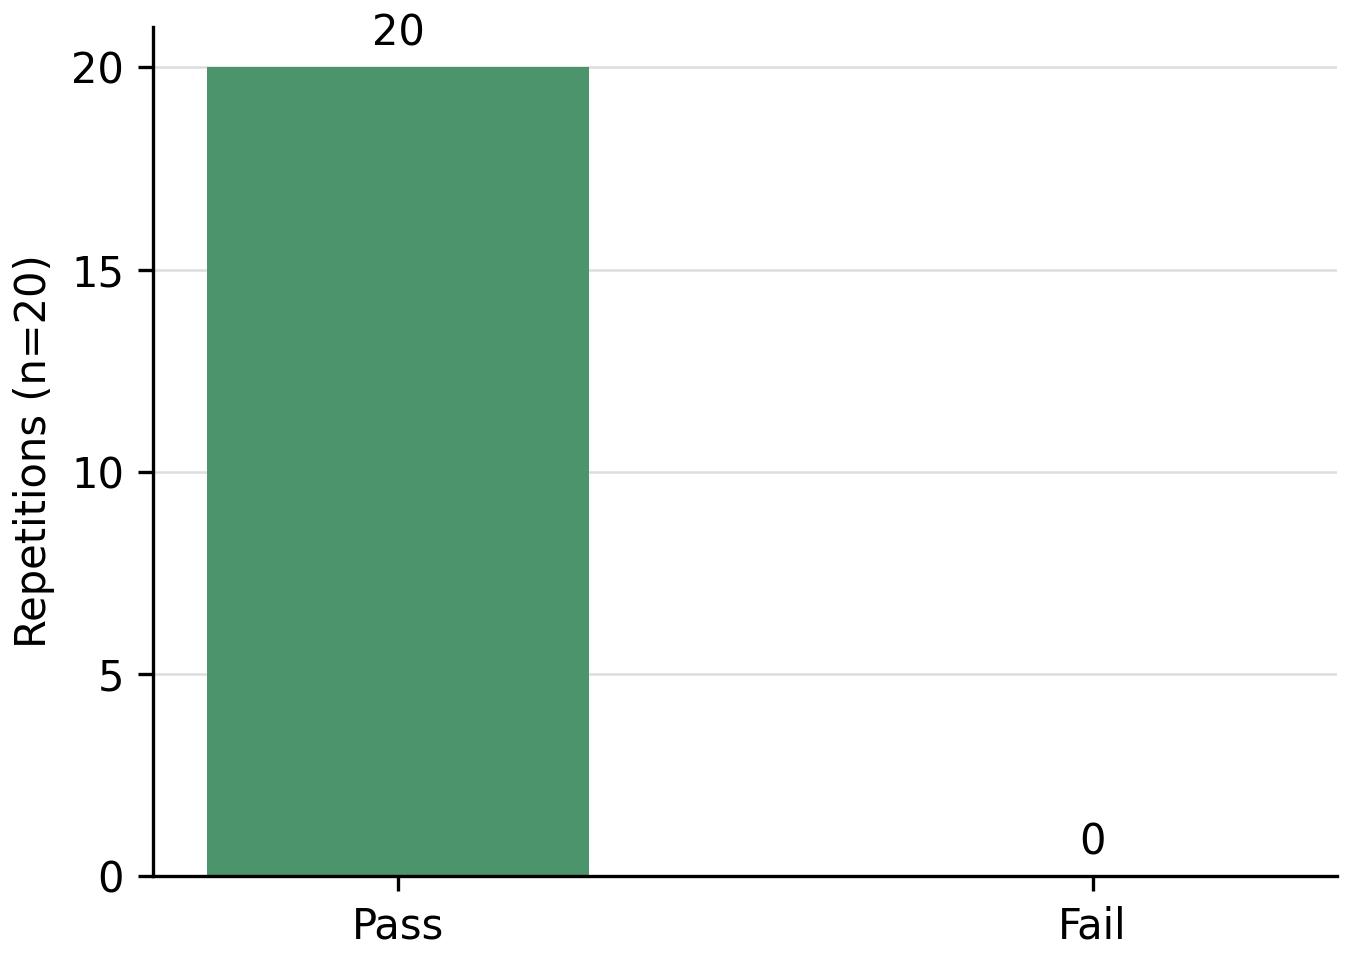
\includegraphics[width=0.94\linewidth]{../results/fig_correctness.png}
  \caption{Count-based correctness repetitions: 20 passes and zero failures.}
  \label{fig:correctness}
\end{figure}

\subsection{Owner Throughput}
The owner averaged 577,652,880 API calls/s with stealing disabled (standard deviation 5,605,951; 95\% confidence interval 575,029,244--580,276,515). At the 1\% target, which achieved 0.90\%, the mean was 532,258,995 calls/s, 7.9\% below baseline. The 5\% target achieved 5.38\% and averaged 531,346,977 calls/s (8.0\% lower). At the 10\% target, the achieved rate was 5.40\% and the mean was 527,109,160 calls/s (8.7\% lower). The 20\% target achieved 5.39\% and averaged 529,463,453 calls/s (8.3\% lower).

The largest difference is between the zero-steal run and the first nonzero setting. At achieved rates near 5.4\%, the three higher targets produced means from 527.11 to 531.35 million calls per second. Their confidence intervals overlap. Since the achieved rates were nearly identical, these means do not show a performance trend from 5\% to 20\% stealing.

\begin{table*}[t]
\centering
\caption{Owner throughput under calibrated target steal rates.}
\label{tab:throughput}
\resizebox{\textwidth}{!}{%
\begin{tabular}{rrrr}
\toprule
Steal rate & Owner ops/s (mean $\pm$ SD) & Relative to 0\% & 95\% CI \\
\midrule
0\% & 577,652,880 $\pm$ 5,605,951 & 100.0\% & [575,029,244, 580,276,515] \\
1\% & 532,258,995 $\pm$ 2,820,458 & 92.1\% & [530,938,995, 533,578,995] \\
5\% & 531,346,976 $\pm$ 803,006 & 92.0\% & [530,971,162, 531,722,791] \\
10\% & 527,109,160 $\pm$ 7,806,288 & 91.3\% & [523,455,747, 530,762,573] \\
20\% & 529,463,453 $\pm$ 1,772,641 & 91.7\% & [528,633,841, 530,293,065] \\
\bottomrule
\end{tabular}}
\end{table*}


\begin{figure}[t]
  \centering
  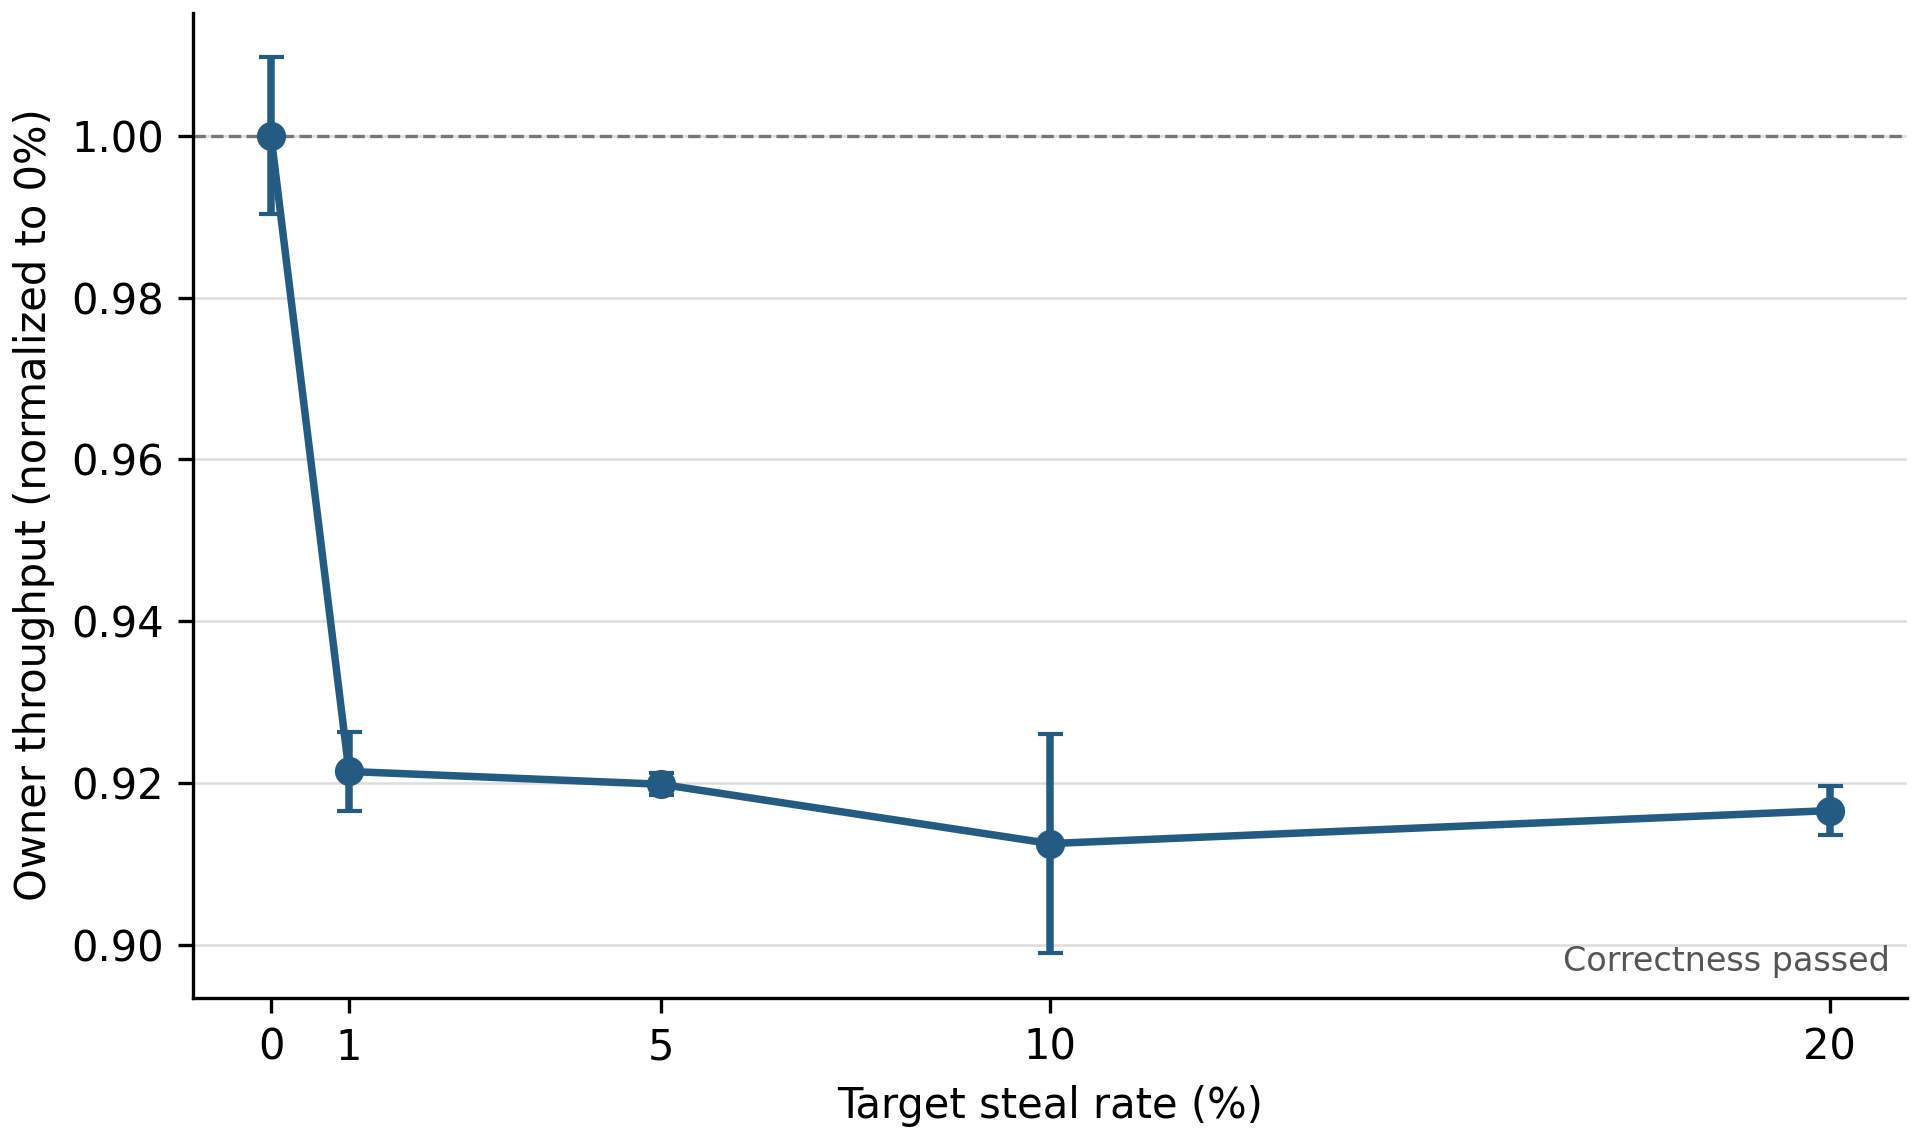
\includegraphics[width=0.98\linewidth]{../results/fig_throughput_vs_stealrate.png}
  \caption{Owner throughput normalized to the zero-steal mean. The x-axis labels are requested targets; achieved percentages are listed in the text and calibration data. Error bars show sample standard deviation.}
  \label{fig:throughput}
\end{figure}

\begin{table}[t]
\centering
\caption{Task-transfer correctness repetitions.}
\label{tab:correctness}
\begin{tabular}{lrr}
\toprule
Outcome & Count & Repetitions \\
\midrule
Pass & 20 & 20 \\
Fail & 0 & 20 \\
\bottomrule
\end{tabular}
\end{table}


\subsection{Calibration Results}
The 1\% target was approached with a mean measured achieved fraction of 0.899\%, and the 5\% target was approached at 5.380\%. The 10\% and 20\% settings selected spin delays of approximately 2 ns and 1 ns, respectively, but both produced approximately 5.4\% achieved steals in timed runs. These small delay values represent the effective limit of this calibration/workload combination, not a proven saturation limit of BWoS itself. Other queue occupancy patterns, owner ratios, processor placements, or implementation versions might support different achieved fractions.

The achieved-rate measurements help explain the shape of the throughput graph. The three higher requested values do not correspond to three increasingly intense concurrent-steal conditions. Instead, they are three attempts to drive one owner--thief queue near or beyond the observed range of the harness. The throughput evidence therefore supports a comparison of no thief calls, light successful stealing, and a roughly 5.4\% contention region. It does not support a claim about a 20\% actual stolen fraction.

\section{Analysis and Parallel-Computing Implications}
\subsection{What the Throughput Change Indicates}
Owner throughput fell as soon as the thief began polling and stealing. This is in line with the problem BWoS is designed to address: even a small amount of stealing can interfere with the queue owner \cite{wang2023bwos}. BWoS separates owner and thief work across blocks to reduce shared synchronization on common operations. My measurements do not show which mechanism accounts for the observed drop. Metadata traffic, block transitions, and the thief's polling may all contribute.

\subsection{Code-Level Comparison with the Original Paper}
The timed loop pushes 768 items and then makes 768 pop calls; meanwhile, the thief repeatedly calls \texttt{steal\_front}. A one-item push/pop cycle gave the thief little opportunity to steal in preliminary runs, so I changed the owner to work in bursts that span three blocks. This makes the owner--thief interaction visible, but also means the result depends on the burst size and block availability. With one queue and one thief, the benchmark says nothing about how a runtime chooses victims or schedules tasks across a pool.

The paper's single-queue test instead fills and drains an 8K-entry queue with eight BWoS blocks, varies the put/get ratio and thief idle time, and reports combined put, get, and steal throughput. My timed queue has four 256-entry blocks, and I count only owner calls. That count includes failed push retries and pops that return empty. I define achieved stealing as successful steals per owner transaction, not the share of all enqueued tasks transferred. These differences make the numbers incomparable: the local 7.9--8.7\% owner-call drop is not the same measure as the paper's 0.53\% combined-throughput drop at 20\% stolen work.

The comparison is therefore qualitative. I observed lower owner throughput with an active thief, which is consistent with the paper's motivation. But the zero-steal thief sleeps while the other conditions use a spin loop, so queue contention is mixed with the cost of keeping a CPU busy. I also have no alternative queue implementation measured on the same machine. The result cannot tell whether BWoS handles interference better than another algorithm.

The calibration changed only the thief's spin delay; the owner's burst size and the queue configuration stayed fixed. Reducing the delay stopped increasing the achieved rate, which leveled off near 5.4\%. That ceiling may reflect intermittent work availability, the single thief, or the calibration method; this experiment cannot separate them. It should not be treated as a limit of BWoS. A useful next test would vary burst size and block capacity separately and record both steal attempts and successful transfers.

The paper provides the algorithmic argument and server-scale results; this experiment records how one C++ port behaved under a specific M4 workload. A closer replication would need to match the queue size, block count, fill/drain pattern, steal-rate definition, and throughput counter. To test whether BWoS has an advantage, it would also need a competing queue measured under the same conditions.

At the 0.90\% achieved rate, owner throughput was about 7.9\% below baseline. That is an observation for this setup, not a per-steal cost estimate. It may include cache-coherence effects, spin-loop activity, or changes in system state. Since threads were not pinned and each sample lasted two seconds, a follow-up should use longer runs, randomized trial order, and stable queue occupancy.

At the three highest targets, the owner mean stayed near 91--92\% of baseline, but achieved stealing stayed near 5.4\% in all three cases. The similar means therefore reflect repeated measurements at about the same contention level. They say nothing about owner throughput at actual 10\% or 20\% stealing, both of which the paper measured \cite{wang2023bwos}.

\subsection{Throughput, Work, and Useful Progress}
The measured unit is an API call, not a completed task or unit of useful computation. The owner throughput counter increments for push and pop calls; a push retry on a full queue is counted as an operation. A steal that succeeds removes an item from the owner-visible queue, but the owner still executes its paired pop call, which may return empty. As a result, the metric captures queue-call activity under interference, not total tasks processed per second. An application study should separately count successful puts, successful gets, successful steals, task completion, failed/retried operations, and useful work time.

This distinction matters when comparing implementations. An algorithm could increase API calls/s by returning empty more quickly, even if useful completed tasks/s does not improve. Conversely, a batched strategy may perform fewer calls while moving more tasks per call. The paper's microbenchmark reports a sum of put, get, and steal operation throughputs for its queue tests, whereas this project reports owner calls only. The counters and denominators differ. The local numbers must not be placed beside the paper's throughput graph as if they measured the same quantity.

The burst workload also illustrates a practical tuning issue. If too little work is outstanding, the thief may have nothing available at the old end of the queue. Larger bursts expose more work, but they change how often the queue crosses block boundaries. Task granularity, occupancy, and block size therefore affect both the opportunity to steal and the synchronization the queue performs.

\subsection{Tuning and Calibration}
The calibration reached the 1\% and 5\% targets but not the two higher targets. At the shortest requested delays, the achieved rate remained near 5.4\%. A single thief may have reached its practical limit under this workload, or the burst pattern may have limited the work available to steal. The data do not distinguish these possibilities. The selected 1--2 ns delays are spin-loop targets, not precise pauses: clock reads, instructions, and scheduling all add time.

In a follow-up, I would keep separate counts for attempts, successful steals per owner transaction, and the fraction of submitted tasks stolen. Recording queue occupancy would help explain why an attempt succeeds or fails. I would also vary the owner's put/get ratio independently of thief delay, as in the paper's single-queue experiment, to see whether a sustained backlog makes higher rates possible.

The queue parameters should also be swept carefully. The correctness test uses four blocks of eight entries to keep the task-transfer test small. The throughput queue uses four blocks of 256 entries and pushes 768 items per burst. These values differ from the paper's eight blocks and 8K-entry capacity. A controlled block-size study could vary block count, block capacity, and burst size while holding total capacity or outstanding work constant. Such a study would test whether the observed calibration ceiling is tied to block availability. A parameter sweep must report memory footprint and task availability, not only raw operations per second.

\subsection{Scaling and Efficiency}
No strong-scaling or weak-scaling claim can be drawn from two worker threads. Strong scaling would keep total work fixed while increasing worker count and measure speedup $S_p=T_1/T_p$ and efficiency $E_p=S_p/p$. Weak scaling would keep work per worker constant and measure how total work changes with worker count. The current test has one owner queue and one thief, no victim pool, and no application tasks with a defined computation cost. It cannot measure these scaling indicators.

A useful scaling study would start with single-queue owner baselines, then add workers while holding queue capacity, task size, and outstanding work constant. It should record aggregate task throughput, per-owner throughput, steal success, idle time, queue occupancy, and latency. Repeated measurements across core counts would show scaling and efficiency; a separate multi-socket machine would be needed to study NUMA effects.

\section{Threats to Validity}
\subsection{Construct Validity}
The benchmark measures owner API calls per second. It counts failed push retries and pop calls that return empty, so it should not be read as tasks completed per second. The workload is a repeated push burst followed by a pop burst; it has no application work or task-completion latency. I define the achieved steal rate as successful steals divided by owner transactions. A different denominator, such as all successfully enqueued items, would give a different percentage.

The 10\% and 20\% labels are requested settings, not achieved rates: both produced about 5.4\%. Likewise, the correctness check compares totals only. It can miss a duplicate paired with a lost ID and does not explore all possible schedules. The paper's GenMC results concern its modeled C implementation, so they do not prove this stdexec port correct.

\subsection{Internal Validity}
The zero-steal thief waits; the other thief configurations spin between calls. That difference affects CPU use and scheduling as well as queue contention, so the throughput drop cannot be attributed to queue metadata alone. Threads were not pinned, and I did not record frequency or thermal state. Each sample lasted two seconds, and the five settings ran in ascending order without randomization. Background activity or heating could therefore influence the later measurements. Repeating in randomized order and across fresh process launches would help separate those effects.

\subsection{External Validity}
The M4 laptop does not match the paper's two 88-hyperthread x86 systems or its 96-core Arm server. It has unified memory, and this experiment uses one queue and two threads; there is no multi-socket NUMA placement or pool of queues. The results should not be generalized to server hardware or a production runtime.

I tested stdexec's C++ port, fetched from its changing \texttt{main} branch and recorded at commit \texttt{3258236616e1}. Its implementation can differ from the paper's C code. The experiment also has no competing queue baseline, so it cannot show that BWoS outperforms ABP or another algorithm on the M4. It measures neither application throughput nor energy, utilization, or task latency.

\subsection{Statistical and Reproducibility Limits}
There are 20 measurements per setting, all from one benchmark run. The confidence intervals summarize variation within that run; they do not capture day-to-day changes or guarantee independent samples. I did not perform a hypothesis test. The source commit, compiler version, raw log, CSV files, and plots are retained with the project. A clean rebuild requires network access for FetchContent and the Python plotting dependencies. Since the dependency follows stdexec's \texttt{main} branch, future runs should pin or record their resolved commit.

\section{Conclusion and Future Work}
I tested stdexec's LIFO BWoS queue on an M4 using one owner and one thief. The count check passed in all 20 runs. Owner throughput averaged 577.65 million API calls/s with stealing disabled, 532.26 million at an achieved 0.90\% steal rate, and between 527.11 and 531.35 million at achieved rates near 5.4\%. The requested 10\% and 20\% rates were not reached.

The main lesson from this experiment is about measurement: the target rate, achieved rate, and throughput counter all need to be stated to interpret the result. I initially expected five distinct steal conditions, but the upper three targets produced essentially the same achieved rate. The data show that this workload's owner throughput was lower when the thief was active; they do not show how BWoS compares with another queue or how it scales to more workers.

For a follow-up, I would first improve rate control and keep queue occupancy steadier while changing the owner-to-thief balance. I would record attempts, successful steals, and task IDs separately, randomize run order, and compare stdexec with at least one baseline. Only after that would I expand to more worker counts. Evaluating NUMA behavior would require a multi-socket machine.

\section*{Code and Data Availability}
The benchmark source, build and export scripts, raw log, and generated result files are maintained in the project repository \cite{aibak2026bwos}. The run-specific stdexec commit and compiler details are recorded with the methods file. The reported measurements correspond to that recorded run; rerunning against a later stdexec revision may produce different results.

\bibliographystyle{IEEEtran}
\bibliography{references}
\end{document}
